\documentclass{gmto}

\usepackage{amsmath}

\DocID{GMT-XXX-\#\#\#\#}
\DocVersion{1.0}
\DocStatus{Draft}

\addbibresource{gmt.bib}

\title{Natural Seeing Observatory Performance Mode Integrated Model Description}
%\subtitle{}
\author{R. Conan, R. Romano, C. Dribusch, H, Fitzpatrick}
\date{\today}

\begin{document}

\maketitle

\clearpage

\section*{Signatures}
\vspace{1cm}
\subsection*{Author}
\vspace{1.5cm}
%\tabulinesep=1em
\begin{tabu} to \linewidth {X[3,l]X[1,l]}
  \rule{\linewidth}{.1pt} & \rule{\linewidth}{.1pt} \\
  Name, title & Date
\end{tabu}
\vspace{1.5cm}
\subsection*{Approvers}
\vspace{1.5cm}
%\tabulinesep=1em
\begin{tabu} to \linewidth {X[3,l]X[1,l]}
  \rule{\linewidth}{.1pt} & \rule{\linewidth}{.1pt} \\
  Name, title & Date \\[1cm]
  \rule{\linewidth}{.1pt} & \rule{\linewidth}{.1pt} \\
  Name, title & Date
\end{tabu}

\clearpage

\section*{Revision Log}

\begin{revisions}
  1.0 & \today & All & None & Initial version & Author \\  
\end{revisions}

\clearpage

\tableofcontents
\listoffigures
\listoftables

\clearpage

\section{Purpose}
\label{sec:purpose}

This document describe the GMT integrated model for the Natural Seeing
Observatory performance mode\cite{ORD}.

\section{Introduction}
\label{sec:introduction}

The integrated model is made of 3 main models of the telescope:
\begin{enumerate}
\item the finite element model of the telescope (FEM),
\item the optical model,
\item the control systems.
\end{enumerate}

In addition, other models are used to compute the disturbances applied to the
integrated model like the atmospheric turbulence model, the computational fluid
dynamics model that computes the dome seeing and the wind pressure exerted on
the telescope, the heat conjugate transfer model of M1 segments to compute the
segments thermal figure errors ...

\begin{figure}
  \centering
  \includegraphics[width=\textwidth]{/home/rconan/Documents/GMT/Review/ASMFDR/nsiq.png}
  \caption{Natural Seeing image quality error budget.}
  \label{fig:ns-iq}
\end{figure}

\clearpage
\section{Models}
\label{sec:models}

\subsection{Finite element model}
The finite element model of the telescope\cite{ss2fem_Christoph2020} is a single mesh that includes all relevant components of the telescope from the ground up, but excludes the enclosure and nearby buildings and structures. 
The level of fidelity with which the components of the telescope are modeled varies greatly. 
Currently the pier, mount, M1 and M2 are modeled with a relatively high level of detail, but some of the other payloads are represented in a simple fashion that accounts for little more than their mass properties and mounting location. 
The mesh can be configured to represent different pointing angles.
Since the FEM does not account for geometric or material non-linearities, it is essentially a set of second order ordinary differential equations (ODE) relating nodal displacements, velocities and accelerations to
applied forces.
The ODEs can be rewritten in terms of the eigenmodes $\vec q$, which allows to drastically reduce the degrees of freedom and provides a representation that is suitable for frequency and especially time domain simulation.
The ODE of a given eigenmode $q_i$ is written as:
\begin{equation}
  \label{eq:1}
  \ddot q_i + 2\omega_i\zeta\dot q_i + \omega_i^2 q_i = \vec b_i\cdot \vec u,
\end{equation}
where $\omega_i$ is the eigenfrequency, $\zeta$ the damping coefficient, $\vec b_i$
the nodal to modal forces projection vector and $\vec u$ the vector of nodal forces.
The corresponding telescope nodal displacements $\vec y$ are derived from
\begin{equation}
  \label{eq:2}
  \vec y = \sum_i q_i\vec c_i  = \sum_i \vec y_i,
\end{equation}
where $\vec c_i$ is the modal to nodal displacement transformation vector.

The scalar ODE in Eq.~(\ref{eq:1}) is rewritten in the following state space model:
\begin{eqnarray}
  \label{eq:3}
  \dot x_i &=& A_ix_i + B_iu   \\
  y_i &=& C_ix_i,
\end{eqnarray}
with
$$
x_i = \begin{bmatrix}
    q_i \\
    \dot q_i
    \end{bmatrix},
  A_i = \begin{bmatrix}
    0 & 1 \\
    -\omega_i^2 & -2\omega_i\zeta
    \end{bmatrix}  
    ,
    B_i = \begin{bmatrix}
      \vec 0 \\
      \vec b
      \end{bmatrix}
    ,
    C_i = \begin{bmatrix}
      \vec c_i & \vec 0
    \end{bmatrix}
    .
$$
  The continuous state space model is transformed into a discrete state space model
  \begin{eqnarray}
    \label{eq:4a}
  x_i[k+1] &=& A_{i,d} x[k] + B_{i,d} u[k] \\
    \label{eq:4b}
  y_i[k] &=& C_i x_i[k],
  \end{eqnarray}
  with
  $$
  A_{i,d} = \exp(A_i\tau),
   B_{i,d} = A_i^{-1}(A_{i,d}-I)B_i$$
  and $\tau$ is the sample time.
Both $A_{i,d}$\footnote{\url{https://www.wolframalpha.com/input/?i=inverse+\%7B\%7B0\%2C+1\%7D\%2C+\%7B-x\%5E2\%2C+-2yx\%7D\%7D}} and $A_i^{-1}$\footnote{\url{https://www.wolframalpha.com/input/?i=Matrixexp\%5B\%7B\%7B0\%2Ct\%7D\%2C\%7B-tx\%5E2\%2C-2txy\%7D\%7D\%5D}} have a closed-form expression:
\begin{equation}
  \label{eq:5}
  A_{i,d} = \begin{bmatrix}
    {\alpha_+\beta_- + \alpha_-\beta_+ \over 2z_i} & {\beta_- - \beta_+ \over 2z_i} \\
    {\omega_i^2 (\beta_+ - \beta_-) \over 2z_i} & {\alpha_-\beta_- + \alpha_+\beta_+ \over 2z_i}
    \end{bmatrix}
\end{equation}
\begin{equation}
  \label{eq:6}
  A_i^{-1} = \begin{bmatrix}
    -2\zeta\omega_i^{-1} & -\omega_i^{-2} \\
    1 & 0
  \end{bmatrix}  
\end{equation}
with $z_i=\omega_i^2\sqrt{\zeta^2-1}$, $\alpha_-=z_i-\omega_i\zeta$,
$\alpha_+=z_i+\omega_i\zeta$, $\beta_-=\exp(\tau\alpha_-)$,
$\beta_+=\exp(-\tau\alpha_+)$.
Thanks to the orthogonality of the eigenmodes $q_i$, the discrete state space
models given by Eq.~(\ref{eq:4a}) and Eq.~(\ref{eq:4b}) are computed in parallel for all the modes of
the system.

The eigenmodes of the telescope FEM\cite{} have been computed for all the modes
up to a eigenfrequency of 2,000Hz leading to a total of 13,381 modes(Fig.~\ref{fig:fem-eig-val}).
\begin{figure}
  \centering
  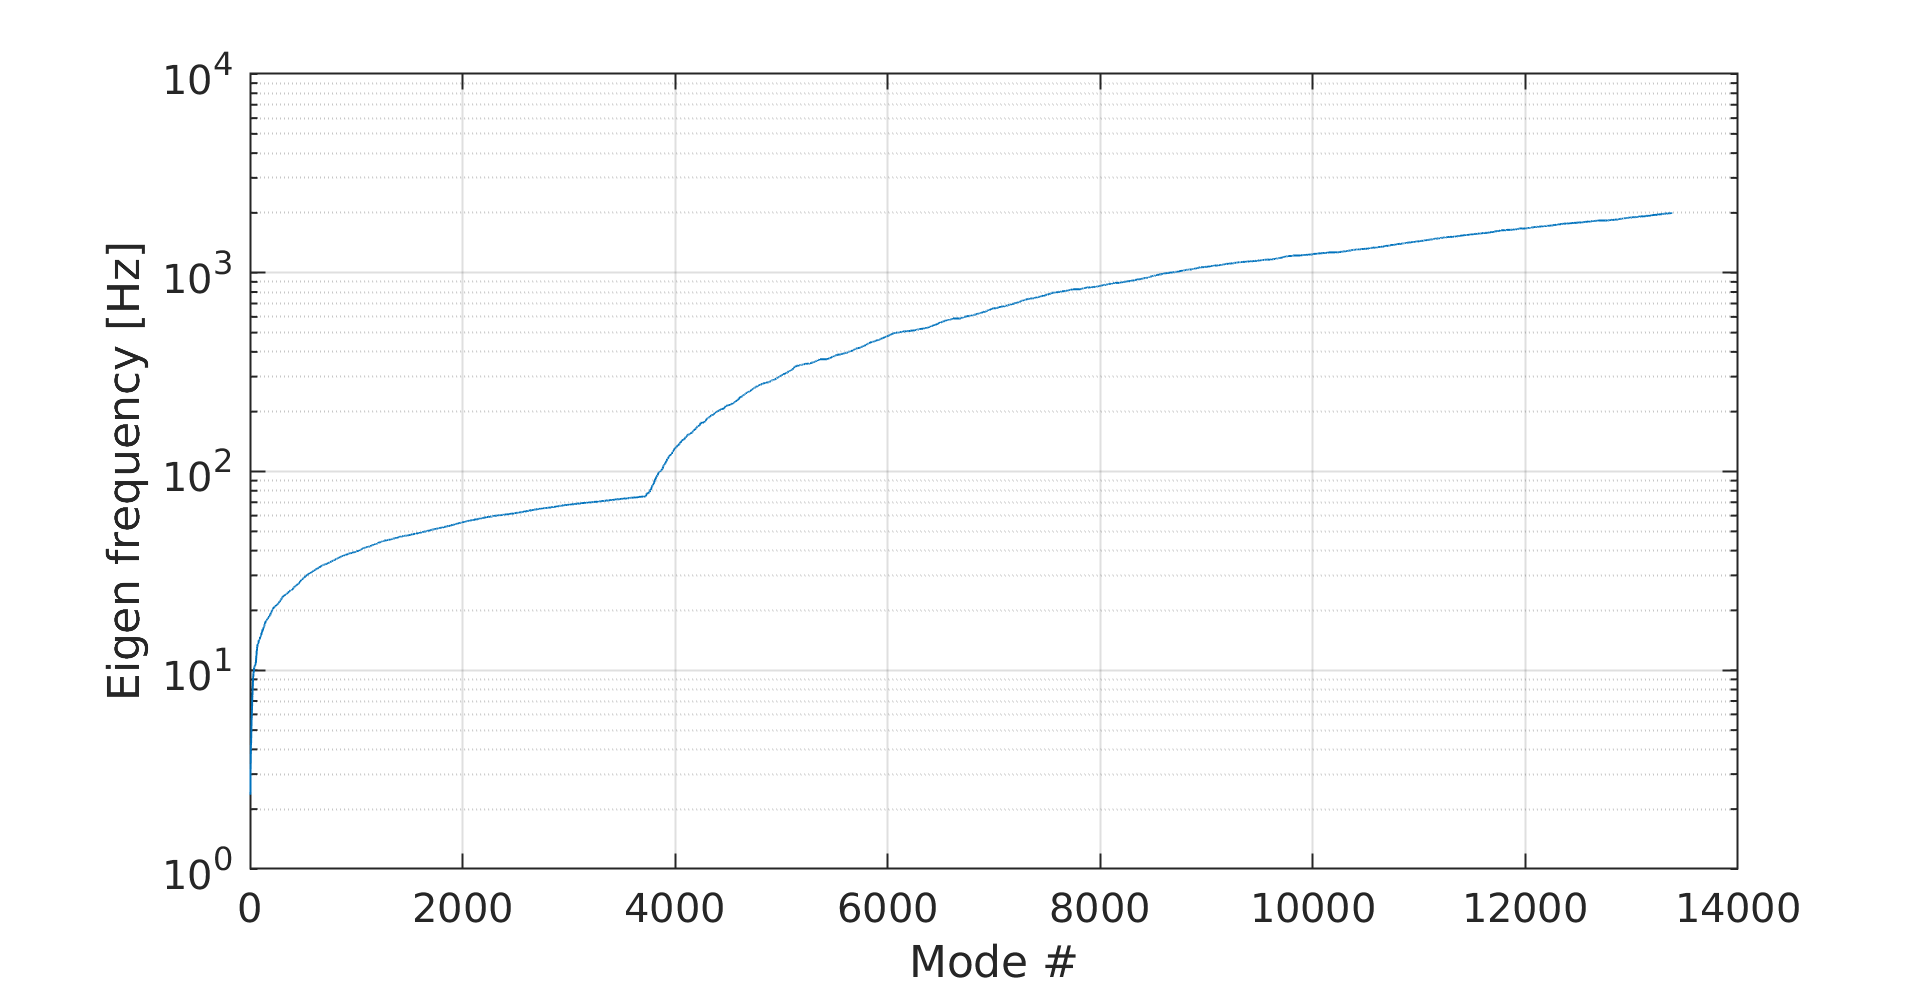
\includegraphics[width=0.7\linewidth]{modal_state_space_model_2ndOrder_2000Hz.png}
  \caption{Telescope FEM eigenfrequencies as a function of the eigenmodes
    number.}
  \label{fig:fem-eig-val}
\end{figure}
To reduce the computational burden, the number of modes of the system is reduced by
thresholding the Hankel singular values of the system.
The state space model is set with a modal damping coefficient $\zeta=2$\% and a
sampling rate $\tau=1$ms. 

A set of inputs and outputs are added to the FEM in order to apply
forces and moments to the model and to get the corresponding node displacements.
The inputs forces and moments are
\begin{description}
\item[the wind load forces](Sec.~\ref{sec:cfd}) applied to
  \begin{itemize}
  \item   the mount top-end, trusses, C-Ring and GIR,
  \item  M1 segment cells, mirrors and mirror covers,
  \item  M2 segments,
  \end{itemize}
\item[the mount drive torques] on the elevation, azimuth and GIR axes,
\item[M1] hardpoints and support actuator forces,
\item[M2] positionner and FSM actuator forces.
\end{description}
The outputs nodes displacements are
\begin{description}
\item[the mount encoder angles] of the elevation, azimuth and GIR axes,
\item[M1]
  \begin{itemize}
  \item hardpoint displacement,
  \item segment rigid body motions,
  \item segment surface deformations,
  \end{itemize}
\item[M2]
  \begin{itemize}
  \item positionner and FSM actuator displacements,
  \item segment rigid body motions,
  \item segment surface deformations,
  \end{itemize}
\end{description}

ODC model integration\cite{mount_pdr_iv}

FEM to state space model\cite{ss2fem_Christoph2020}

The FEM of the telescope is composed of the FEM of the mount, of M1 and of M2.
It has been configured for 3 elevation angles: 90, 60 and 30 degrees.

To add for each elevation angle:
\begin{itemize}
\item table of 1st few eigenfrequencies
\item plot of modes vs. eigenfrequencies
\item plot of modes vs. Hankel  singular values
\item plot of some transfer functions before and after model reduction
\end{itemize}


\subsubsection{Mount FEM}
\label{sec:mount-fem}

ODC\cite{}

\subsubsection{M1 FEM}
\label{sec:m1-fem}

\paragraph{Gravity support forces}

\paragraph{M1 eigenmodes}

The telescope FEM in its state space representation provides as outputs the
displacement of nodes on the surface of M1 segments as well as the 6 rigid body
motions of the segments.
Both the surface deformations and the rigid body motions of the segments are
moved over to the optical model (Sec.~\ref{sec:optics}).
The optical model then updates the state of M1 segments before proceeding to ray
tracing through the telescope.

In the optical model, the surface deformations of the segments is superimposed
onto the rigid body motions i.e. the surfaces are defined in the coordinate system
associated to the rigid body motions whereas in the FEM the surfaces are defined with
respect to the coordinate system of each segment\cite{GMTO.CoordinateSystems}.

Assuming the vector of translation $\vec t_i$, the rotation matrix $R_i$ and the
coordinate vector of node $k$ $\vec n_{i,k}$ at the surface of M1 segment \#$i$, the following
geometric transformation is applied to the nodes
\begin{equation}
  \label{eq:7}
  \vec n_{i,k} \leftarrow R_i^{-1}(\vec n_{i,k}-\vec t_i).
\end{equation}
Based of the lateral stiffness of M1 mirrors, it is assumed that $\vec
n_{i,k}-\vec t_i \simeq [0,0,\delta_{z,k}]^T$ and Eq.~(\ref{eq:7}) simplifies to
\begin{equation}
  \label{eq:8}
  \vec n_{i,k} \leftarrow \delta_{z,k} \vec r_{i,3} 
\end{equation}
where $\vec r_{i,3} = [r_{i,13},r_{i,23},r_{i,33}]^T$ is the 3rd column of $R_i^{-1}$.
Further neglecting the lateral surface shears of the mirror, the surface
deformation of segment $i$ is finally written as
\begin{equation}
  \label{eq:8}
  S_i = [\delta_{z,k}r_{i,33}]^T,\forall k \in i.
\end{equation}

To reduce the amount of data that is given to the optical model, the surface
$S_i$ is projected on the M1 segment eigenmodes $B_i$ like so $b_i = B_i^TS_i$
where $B_i$ is derived from the singular values decomposition of the sensitivity
matrix $F_i$ that relates actuator cylinder forces to surface deformations, $F_i
= U_i \Lambda_i V_i^T$.
The 6 lowest eigen values correspond to the 6 rigid body motions that have been
filtered out of each influence function in $F_i$ and $B_i$ is given by $U_i$
with the 6 eigenmodes corresponding to the 6 lowest eigen values removed.

Using $B_i$ as the modal basis for M1 segments in the optical model, we can compute
a calibration matrix $D$ that relates the mode coefficients $b$ to the WFS
measurements $s$, $s=Db$.
The actuator forces are related to the modes coefficients with $f_i =
V_i\Lambda_i^{-1}b_i = V_i\Lambda_i^{-1}D^\dagger s$ and these forces must bear
no loads on the segments hardpoints as any hardpoints load would in turn induce
stresses into the glass.
It is worth noting that the feedback force measurements from the hardpoints load cells
would capture any spurious forces and off-load them to the actuators hence
``tainting'' the M1 surface deformations with hardpoint footprints.
In order to avoid such contamination from the hardpoint, a new segment modal
basis is derived in the following such as the associated forces lay in the null
space of the hardpoints.

The derivation starts from the gain $G$ of the FEM static solution reduced to M1
actuator forces as inputs and hardpoint displacements and M1 surface
deformations as outputs:
\begin{equation}
  \label{eq:9}
  G = \begin{bmatrix}
    G_\beta \\ G_\alpha
  \end{bmatrix},
\end{equation}
where $G_\beta$ and $G_\alpha$ are the gain matrices for the hardpoints and
mirror surface, respectively, from which we compute the singular value
decomposition:
\begin{eqnarray}
  \label{eq:10}
  G_\beta &=& U_\beta\Lambda_\beta V_\beta^T \\
  G_\alpha &=& U_\alpha\Lambda_\alpha V_\alpha^T .
\end{eqnarray}
Both $V_\beta$ and $V_\alpha$ are forces eigen vectors and the hardpoints forces
eigen vectors are filtered out of the mirror surface with
\begin{equation}
  \label{eq:11}
  \bar V_\alpha = V_\alpha - V_\beta V_\beta^T  V_\alpha.
\end{equation}
The hardpoints displacements corresponding to the actuator forces given by $\bar
V_\alpha$ are written
\begin{equation}
  \label{eq:12}
  G_\beta \bar V_\alpha = G_\beta  V_\alpha - G_\beta V_\beta V_\beta^T  V_\alpha = U_\beta\Lambda_\beta V_\beta^T V_\alpha - U_\beta\Lambda_\beta V_\beta^T V_\alpha =0,
\end{equation}
using the orthonormal property of the eigen vectors, $V^TV=I$.
The final eigenmodes are given by the left eigen vectors $U$ of the newly
formed gain matrix $\bar G$,
\begin{equation}
  \label{eq:13}
  \bar G = \bar U_\alpha\Lambda_\alpha V_\alpha^T = U\Lambda V^T.
\end{equation}

\subsubsection{M2 FEM}
\label{sec:m2-fem}


\clearpage
\subsection{Optical model}
\label{sec:optics}

\cite{GMTO.OpticalDesign}

\subsubsection{GMT optical model}
\label{sec:gom}

plot of GMT pupil (M2 baffle (3.6m), M1 drain holes, trusses)

\paragraph{M1 polishing error}

\paragraph{M1 gravity print-through}

\subsubsection{AGWS model}
\label{sec:agws}

\paragraph{SH24}

\paragraph{SH48}

\clearpage
\subsection{Control systems}
\label{sec:control}

Fig.~\ref{fig:ns-ctrl} reproduces the Natural Seeing OPM control block diagram
from the GMT Observatory Architecture Document\cite{OAD}.
\begin{figure}
  \centering
  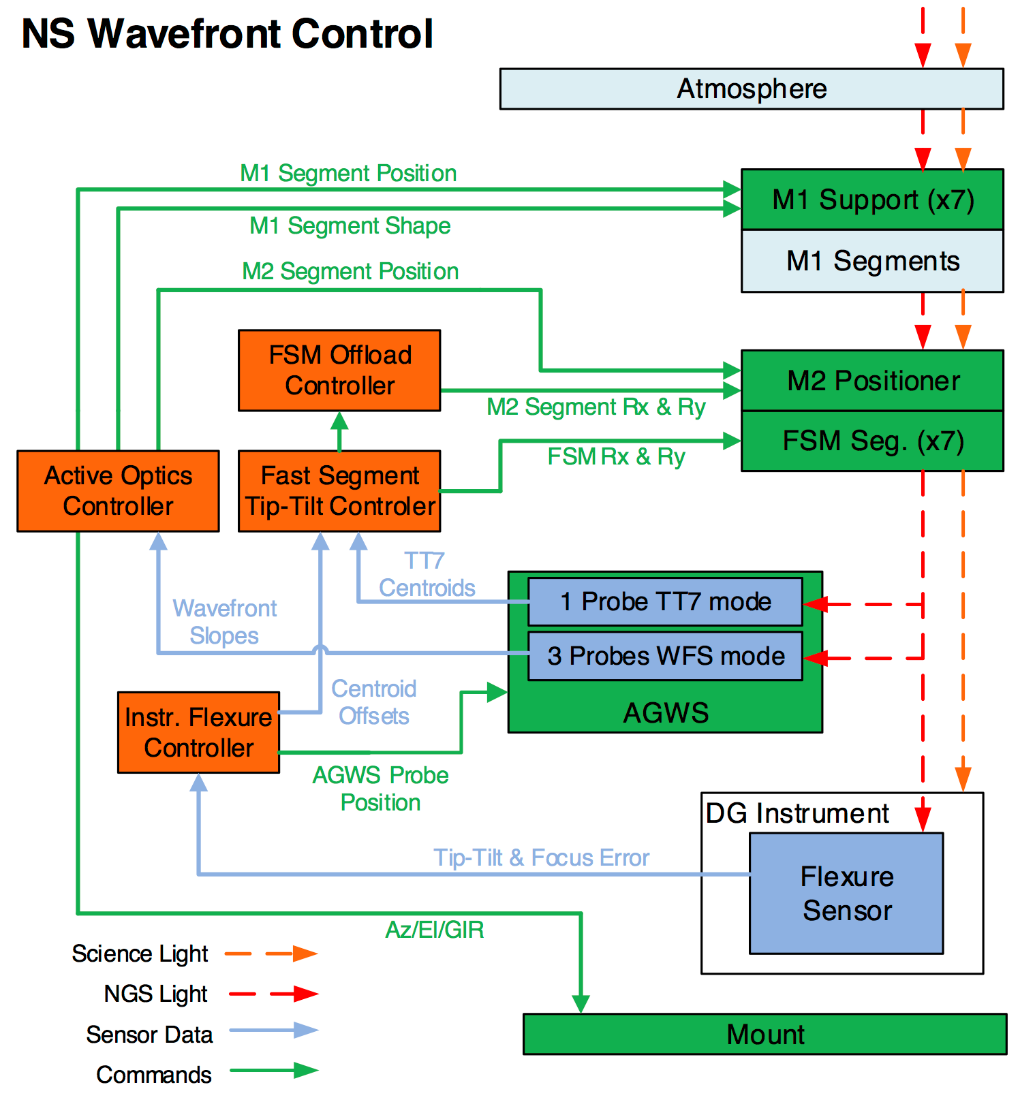
\includegraphics[width=0.8\linewidth]{ns-control.png}
  \caption{Natural Seeing control block diagram.}
  \label{fig:ns-ctrl}
\end{figure}

\subsubsection{Mount controller}
\label{sec:mount-ctrl}

\subsubsection{M1 hardpoints to actuators force loop }
\label{sec:m1-ctrl}

\cite{GMT.DOC.05153}

\subsubsection{M2 controllers}
\label{sec:m2-ctrl}

\cite{GMT.DOC.05154}

\paragraph{M2 positionner controller}

\paragraph{M2 segment piezo--actuators controller}

\subsubsection{Optical feedback loops}
\label{sec:optics-ctrl}

\paragraph{FSM tip--tilt loop}


\paragraph{Active Optics}


\clearpage
\subsection{Disturbances}
\label{sec:disturbances}

\subsubsection{Atmospheric turbulence model}
\label{sec:atm}

validation of the atmospheric model\cite{GMT.DOC.01862}


\subsubsection{Computational fluid dynamics}
\label{sec:cfd}

\paragraph{Dome seeing}

\paragraph{Wind pressure}

\cite{GMTO.DOC.03352}

\subsubsection{M1 heat conjugate transfer model}
\label{sec:m1-hct}

\cite{GMT.DOC.04558,GMT.DOC.04557,GMT.DOC.04894}
\paragraph{Soak error}

\paragraph{Segment core thermal footprints}



\clearpage

\printbibliography

\end{document}
